\documentclass[12pt]{article}
\title{CEG5303 Lab 1 Report}
\author{Group 20 \\MA HAOYUAN (A0279682J)\\SUN CHENCHEN (A0058718U)\\ SUN YIJING (A0279605U)}
\date{\today}

\usepackage{amsmath}
\usepackage{graphicx}
\usepackage{hyperref}
\usepackage[a4paper,margin=1in]{geometry}
\usepackage{setspace}
\usepackage{float}
\usepackage{subcaption}
\usepackage{listings}

\setstretch{1.5}
\hypersetup{colorlinks=true, linkcolor=blue, citecolor=blue}
\bibliographystyle{ieeetr}


\begin{document}
\pagenumbering{roman}
\maketitle

\tableofcontents

\newpage
\pagenumbering{arabic}

\section{Introduction}
In this lab assignment, we modelled quadcopter system using Matlab and simulink following a simplified dynamics model. Various control methods including PID and MPC are realized to control the quadcopter to follow a given trajectory.
The basic dynamics model given by the TA is also refined to
incorporate a more realistic wind dragging effect.

\section{Group: Basic Realization}
\label{sec:basic_realization}
After following instructions in guidance document \cite{lab1_guidance},
we successfully built a drone simulation using PID control method, which can follow the pre-defined simple trajectories
reasonably well.

\subsection{Dynamics}
The drone plant in Simulink implemented the dynamics in Figure \ref{fig:dynamics_model}.
Note the dynamics equation assumes a linear damping term $-\frac{1}{m}D_B\dot{\text{p}}$ with respect to the drone velocity.

% \begin{figure}[H]
%     \centering
%     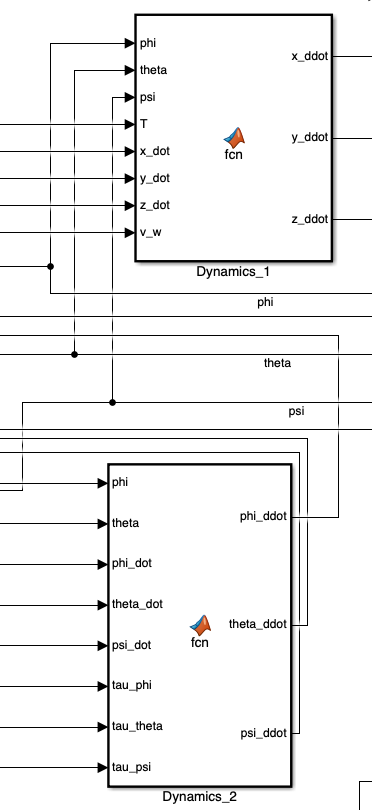
\includegraphics[width=0.4\textwidth]{figures/drone_plant}
%     \caption{part of the drone plant implementing the dynamics}
%     \label{fig:drone_plant}
% \end{figure}

\begin{figure}[H]
    \centering
    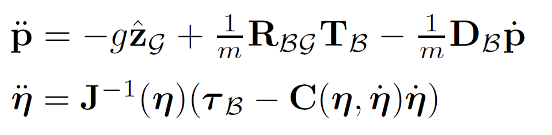
\includegraphics[width=0.5\textwidth]{figures/dynamics_model}
    \caption{drone dynamics equation}
    \label{fig:dynamics_model}
\end{figure}

\subsection{Control}

% The drone control consists of 4 sets of PID parameters (Figure \ref{fig:pid_design})
% \begin{itemize}
%     \item one set \textit{K*\_z} decides the total thrust $T$, to control altitude
%     \item two stage PID to control the $\phi$ and $\theta$ orientation
%           \begin{itemize}
%               \item first stage \textit{K*\_pos} decides the estimated $\phi$ and $\theta$ angle
%               \item second stage \textit{K*\_att} decides the $\tau_\phi$ and $\tau_\theta$ torque output based on the first stage angle
%           \end{itemize}
%     \item one set \textit{K*\_psi} decides the torque $\tau_\psi$, to control the $\psi$ angle
% \end{itemize}


% \begin{figure}[H]
%     \centering
%     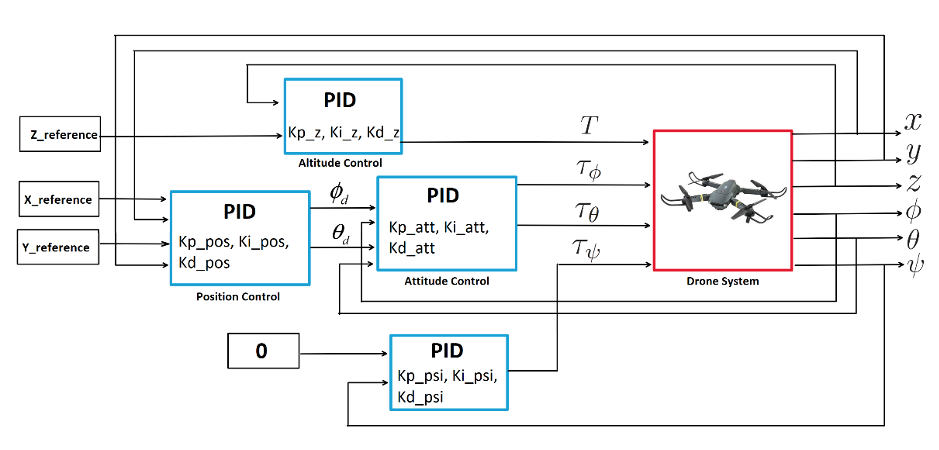
\includegraphics[width=.8\textwidth]{figures/pid_control}
%     \caption{PID control design in Simulink}
%     \label{fig:pid_design}
% \end{figure}

\noindent Our PID control also has a few key assumptions
\begin{itemize}
    \item The generated total thrust $\mathbf{T}$ is always greater than $m \times g$. This is to keep the drone hovering in the air.
    \item There's no max thrust limit imposed on the model, which can be a point for improvment for a more realistic simulation
          %   \begin{figure}[H]
          %       \centering
          %       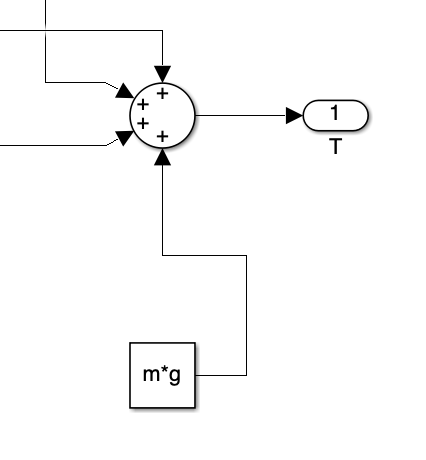
\includegraphics[width=.3\textwidth]{figures/min_thrust}
          %       \caption{Min thrust in Simulink}
          %       \label{fig:min_thrust}
          %   \end{figure}
    \item The estimated $\phi$ and $\theta$ angle by the PID has a limit of $[-4, 4]$ degree.
    \item The max torque can be generated is limited to $[-5, 5] Nm$ in this system.
          % This aims to limit drone's abrupt rotational movement together with the previous constraint
          %   \begin{figure}[H]
          %       \centering
          %       \begin{subfigure}{.4\textwidth}
          %           \centering
          %           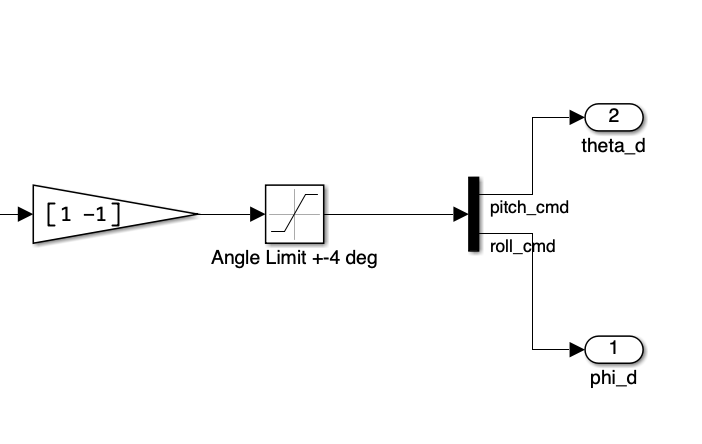
\includegraphics[width=.8\linewidth]{figures/angle_limit}
          %           \caption{Angle limit in Simulink}
          %           \label{fig:angle_limit}
          %       \end{subfigure}
          %       \hspace{.2\textwidth}
          %       \begin{subfigure}{.3\textwidth}
          %           \centering
          %           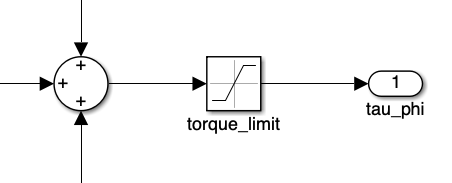
\includegraphics[width=.8\linewidth]{figures/torque_limit}
          %           \caption{Torque limit in Simulink}
          %           \label{fig:torque_limit}
          %       \end{subfigure}
          %       \caption{Angle and torque limits in Simulink}
          %       \label{fig:limits}
          %   \end{figure}
\end{itemize}

\subsection{Parameter Tuning and Evaluations}

After carefully tuning the parameters, we find the following combination that works the best for our evaluation trajectory.

\begin{table}[H]
    \centering
    \begin{tabular}{|l|c|c|c|}
        \hline
                & P    & I   & D   \\
        \hline
        K*\_z   & 5    & 0   & 7   \\
        K*\_pos & 10   & 0   & 2   \\
        K*\_att & 0.03 & 0   & 0.3 \\
        K*\_psi & 1    & 0.1 & 1.5 \\
        \hline
    \end{tabular}
    \caption{Best combination of PID parameters}
    \label{tab:pid}
\end{table}

The system is tested with a reference trajectory of moderate complexity.
The duration of the flight simulation is 120s and the path consists of 5 waypoints.
The \textbf{optimization goal} is to make the drone to reach every destination waypoint, within the time limit, \textbf{as quickly as possible}.
% Once it reaches the waypoint before the next waypoint is genearted, it's expected to stay at the same position.
% Throughout the flight, the drone needs to keep its orientation at close to $\{0, 0, 0\}$ degree.

From Figure \ref{fig:pid_position_evaluation}, it is clear to see that the drone is able to reach the designated waypoints quickly with little overshooting.
It reaches the z reference position much quicker than at the x, y reference position. This is due to no max thrust limit on the z direction, while the max torque limit exists in the system.
The visualization of the drone's flight path is shown in Figure \ref{fig:pid_flight_path}.





\begin{figure}[H]
    \begin{subfigure}{.5\linewidth}
        \centering
        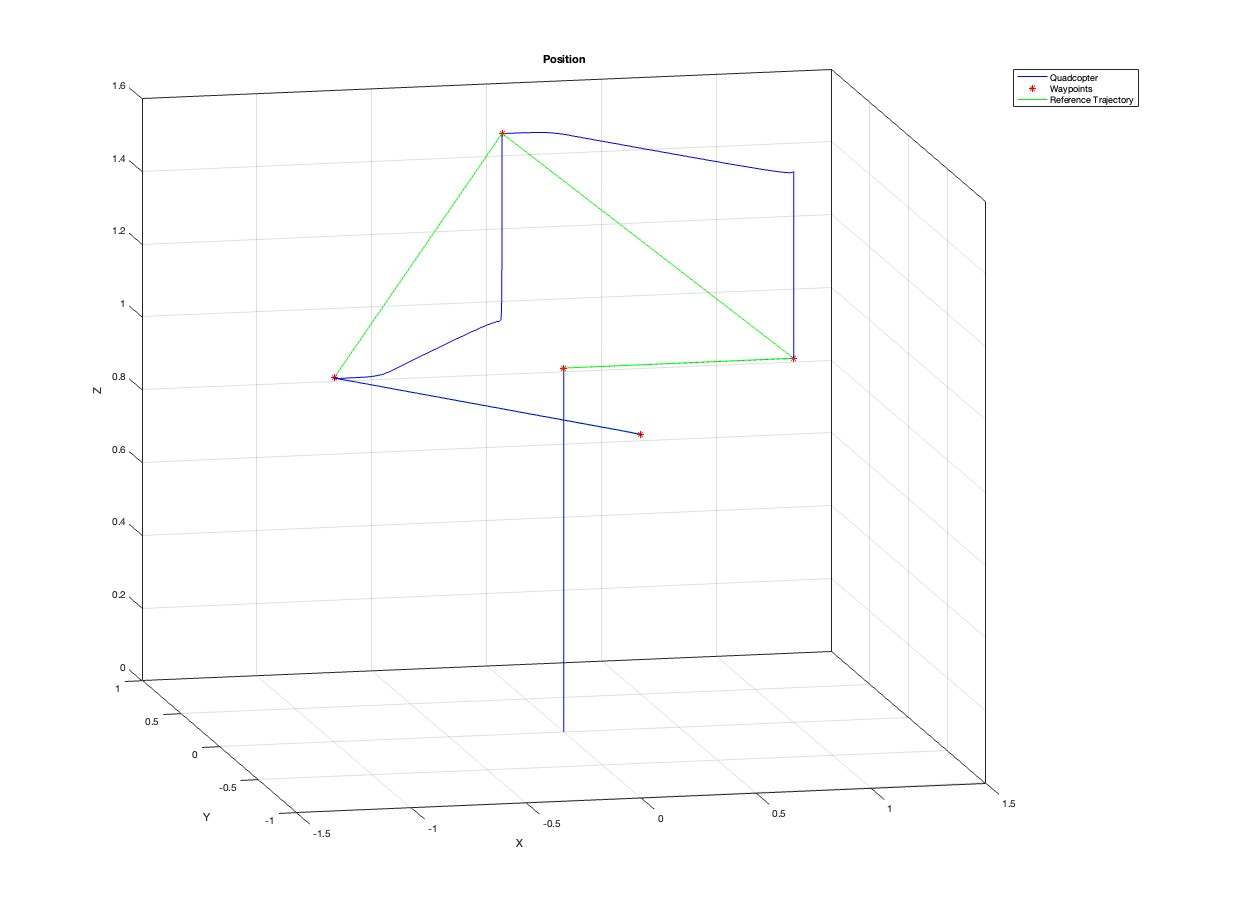
\includegraphics[width=\textwidth]{figures/pid_flight_path.jpg}
        \caption{Flight path}
        \label{fig:pid_flight_path}
    \end{subfigure}
    \begin{subfigure}{.5\linewidth}
        \centering
        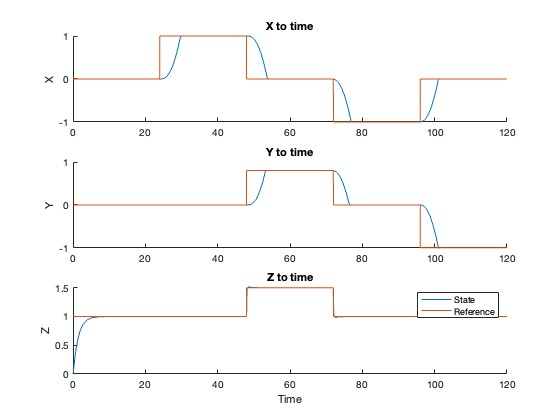
\includegraphics[width=\textwidth]{figures/evaluation_position}
        \caption{Position against reference waypoints}
        \label{fig:pid_position_evaluation}
    \end{subfigure}

    \caption{Flight path analysis}
\end{figure}


\section{Group: Improved Dynamics Model}

\subsection{More realistic air drag force modelling}
As mentioned in Section \ref{sec:basic_realization}, the dynamics model provided in the guidance document assumes the damping effect
linear to the drone's velocity $\dot{\mathbf{p}}$.
Furthermore, the model assumes there's no external wind disturbance. It will be intersting to incorporate
the measured wind disturbance into the modelling, to see how well the PID control method can adapt to it.

According to \cite{cano_quadrotor_nodate}, the following equation can be used to calculate the drag force more accurately.

\begin{align}
    \label{eq:wind_drag_model}
    \mathbf{D}_\mathcal{B} & = \frac{1}{2}\rho_\text{air}\mathbf{C}_\mathcal{B}\mathbf{A}_\mathcal{B}\mathbf{V}^T\mathbf{V}
    % \mathbf{A}_\mathcal{B} & = \begin{bmatrix}A_x & 0 & 0\\0& A_y& 0\\0& 0& A_z\end{bmatrix}                                \\
    % \mathbf{C}_\mathcal{B} & = \begin{bmatrix}C_x & 0 & 0\\0& C_y& 0\\0& 0& C_z\end{bmatrix}
\end{align}

Where $\mathbf{D}_\mathcal{B}$ is the drag force quadcopter experienced in the body frame. $\rho_\text{air}$ is the air density in $[kg/m^3]$, $\mathbf{A}_\mathcal{B}$ is the quadcopter area exposed to the air in body frame in $[m^2]$.
$\mathbf{C}_\mathcal{B}$ is the drag coefficient associated with the quadcopter profile in body frame.
$\mathbf{V} = \mathbf{V}_\text{air} - \dot{\mathbf{p}_\mathcal{B}}$ is the relative velocity between the quadcopter and air flow in $[m/s^2]$

Thus by replacing the original linear drag term, the translational dynamics model now becomes

\begin{equation}
    \ddot{\mathbf{p}} = -g\hat{\mathbf{z}}_{\mathcal{G}} + \frac{1}{m}\mathbf{R}_{\mathcal{BG}}\mathbf{T}_\mathcal{B} + \frac{1}{m}\mathbf{R}_{\mathcal{BG}}\mathbf{D}_\mathcal{B}
\end{equation}

We also assume that, due to the symmetrical profile of the quadcopter, the air drag force will have a net-zero torque with respect to the center of mass.
Thus the rotational dynamics part will not be affected by the introduction of new air drag model.

\subsection{Evaluation}

We modified the code using the new model (Eq. \ref{eq:wind_drag_model}) defined above.
For a more realistic modelling, the newly defined parameter like air drag coefficient, exposed air area etc, are set following the specification for DJI M100, listed in \cite{liuswanto_modelling_2021}

% We first tested out the new model with updated air drag using the original PID combination we obtained in Section \ref{sec:basic_realization}. Comparing to Figure \ref{fig:air_position_evaluation},
% we noticed that the control starts to exhibit symptom of overshooting. This change is especially pronounced on the $\hat{z}$ direction, where the velocity is greater.

% \begin{figure}[H]
%     \centering
%     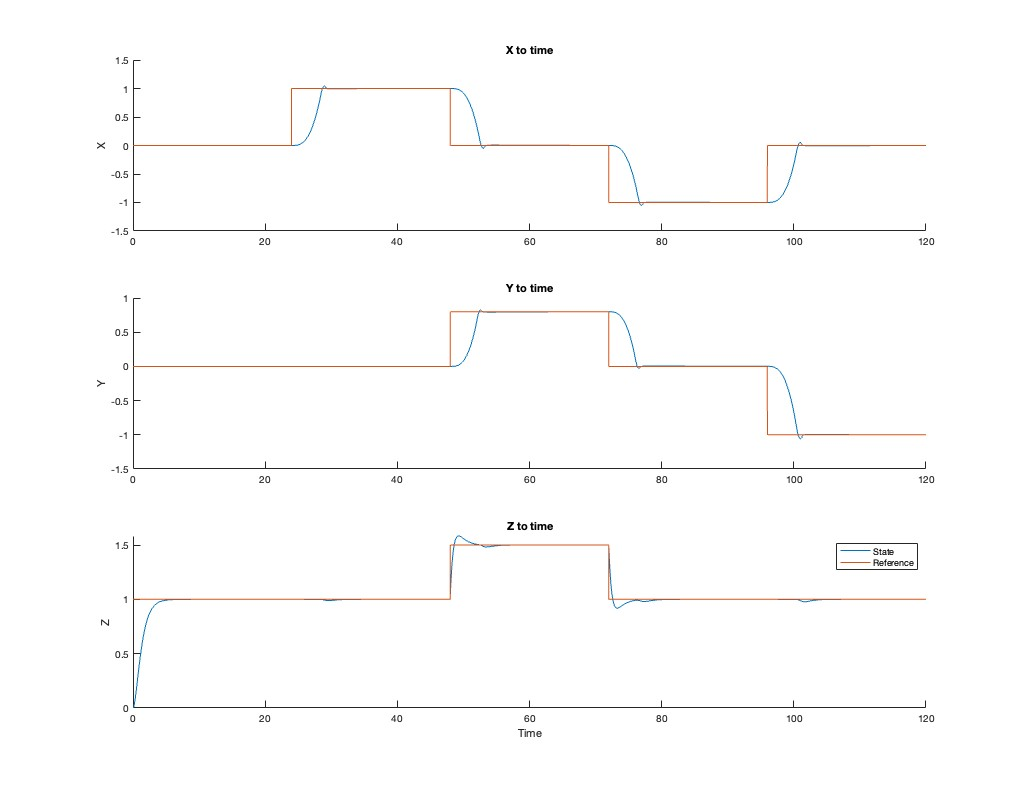
\includegraphics[width=.8\linewidth]{figures/evaluation_position_air}
%     \caption{Drone position against reference waypoints in improved model}
%     \label{fig:air_position_evaluation}
% \end{figure}

To evaluate the effect of wind disturbance. We added a constant horizontal airflow at $\hat{y}$ direction at various speed.
The wind speed ranges from 1 $m/s^2$ to 5 $m/s^2$.

We fine-tune the PID values again and the new optimal combination is as following:

\begin{table}[H]
    \centering
    \begin{tabular}{|l|c|c|c|}
        \hline
                & P    & I    & D   \\
        \hline
        K*\_z   & 30   & 0    & 50  \\
        K*\_pos & 10   & 0.05 & 3   \\
        K*\_att & 0.03 & 0    & 0.4 \\
        K*\_psi & 1    & 0.1  & 1.5 \\
        \hline
    \end{tabular}
    \caption{Best combination of PID parameters for updated air drag model}
    \label{tab:pid_air}
\end{table}
% Comparing to Table \ref{tab:pid}, the new best $P$ and $D$ value are increased for both K*\_z and K*\_pos. Thoug K*\_z increased much more.

% The increase matches with our intuition. Now the air drag force has quadratic relationship with the velocity. Under the same velocity, the resistance force will be greater than before.
% Thus a higher $P$ value is needed. The rate of force change is also much greater than before, hence we will need a larger damping factor $D$ to prevent overshooting as well.

% The position evaluation using the updated PID values can be found in Figure \ref{fig:optimal_air_position_evaluation}. The overshooting is improved under the new set of PID parameters.
% It's worth noting that due to the higher damping factor $D$, the quadcopter now moves to the Z reference position slower than before.
We observed that the quadcopter is able to follow the original trajectory reasonably well under 4 $m/s^2$. Once the wind speed is higher than that,
the original optimal PID parameters will be inadequent to compensate for the stronger external disturbance. This can be seen from the flight trajectory in Figure \ref{fig:pid_flight_path_strong_wind}.

This demonstrates the inherent limiation of PID control methods. It only works well around a fixed environment state, for which it is optimized for.
It could not adapt well to a highly dynamic system.



\begin{figure}[H]
    \centering
    \begin{subfigure}{.5\linewidth}
        \centering
        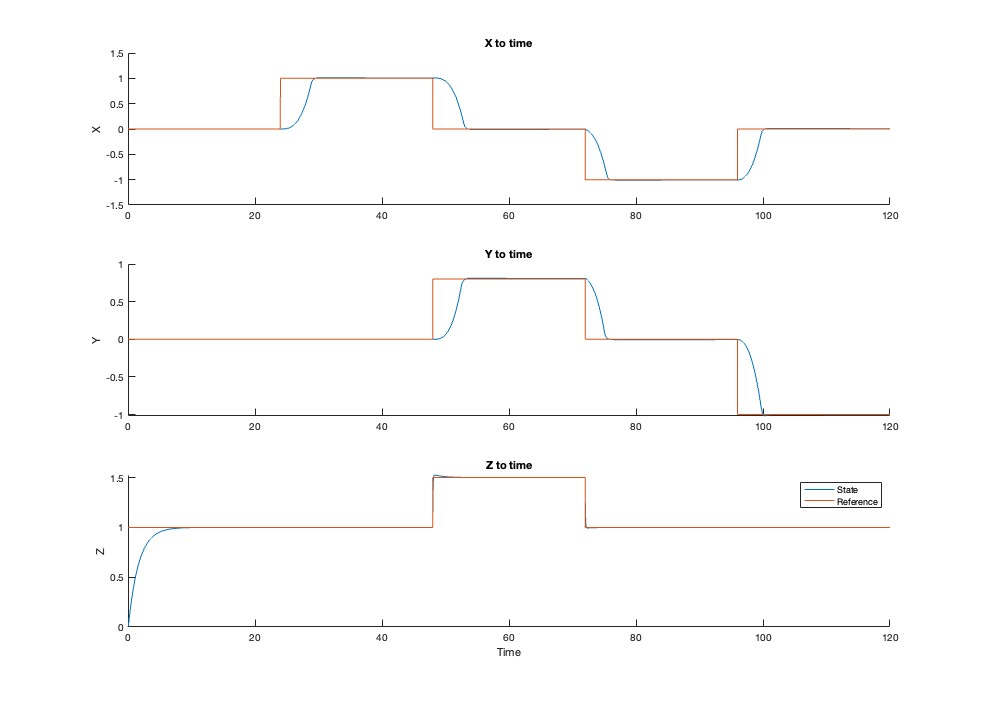
\includegraphics[width=\linewidth]{figures/evaluation_position_air_optimal}
        \caption{Position plot at wind speed 3$m/s$}
        \label{fig:optimal_air_position_evaluation}
    \end{subfigure}
    \begin{subfigure}{.45\linewidth}
        \centering
        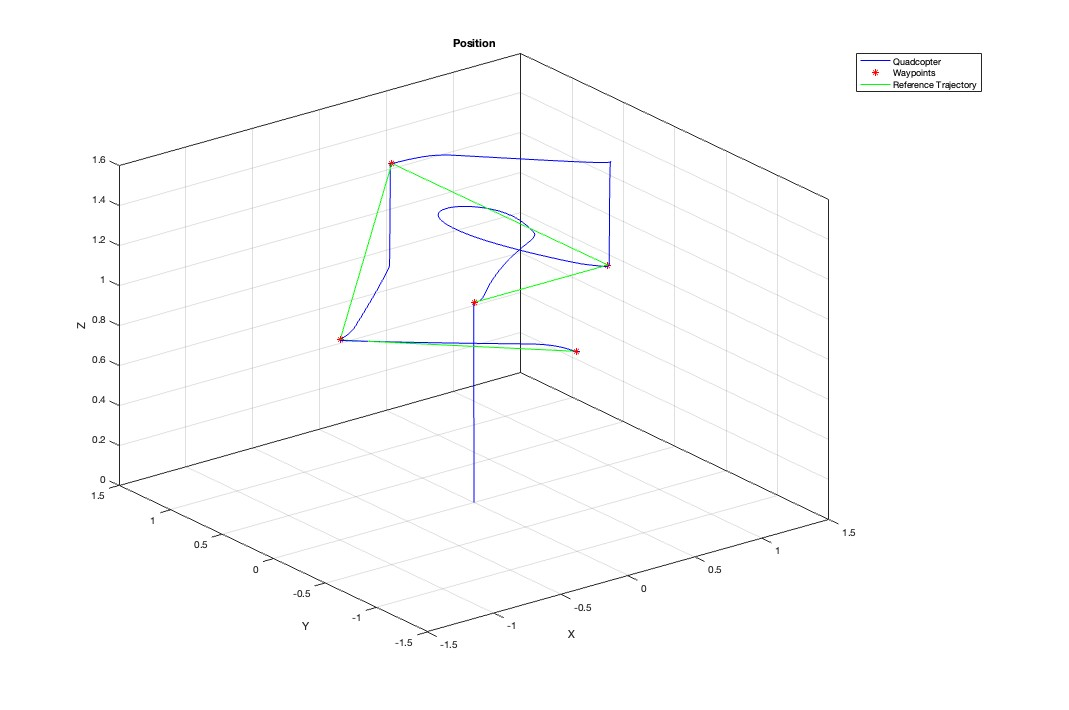
\includegraphics[width=\linewidth]{figures/pid_flight_path_strong_wind}
        \caption{Flight path at wind speed 4.3$m/s$}
        \label{fig:pid_flight_path_strong_wind}
    \end{subfigure}
\end{figure}



\section{[Sun Chenchen]: Model Predictive Control (MPC) with quadcoper}

We decide to try out MPC control to see whether it can control the quadcopter well using the new air drag model.
The code is adapted from the official example in Matlab's Model Predictive Control Toolbox. \cite{mathworks_quadrotor}.
The adaptations includes:

\begin{itemize}
    \item Replace the original dynamics model code with our own
    \item Modify the MPC setup to support measured wind disturbance.
\end{itemize}

\noindent The nonlinear MPC is set up with the following parameters

\begin{itemize}
    \item 12 states and 12 outputs: $x, y, z, , \phi, \theta, \psi, \dot{x}, \dot{y}, \dot{z}, \dot{\phi}, \dot{\theta}, \dot{\psi} $
    \item 4 inputs: squared angular velocity of rotor: $u1, u2, u3,u4$
    \item Timestep: 0.1s; Prediction Horizon: 18; Control Horizon: 2; $\rightarrow$ 1.8s fixed prediction horizon. The simulation runs for 20s.
    \item The objective function only use state $x, y, z, \phi, \theta, \psi$, and input $u1, u2, u3,u4$ to compute the cost. Input weight is set to 0.1 while state weight is 1.
          % \item The target for $\phi, \theta, \psi$ is 0 degree throughout the flight
          % \item The target for input $u1, u2, u3,u4$ is set to keep the quadcopter hovering in the air
\end{itemize}

\subsection{Evaluation of MPC control}

% We first evaluate the effectiveness of MPC control for our model with accurate air drag calculation, using a simple straight line path.
% The simulation in Figure \ref{fig:mpc_evaluation_simple_path} and \ref{fig:mpc_simple_path} shows that the quadcopter is able to track the reference path really well using the MPC method with close to zero overshooting

% \begin{figure}[H]
%     \centering
%     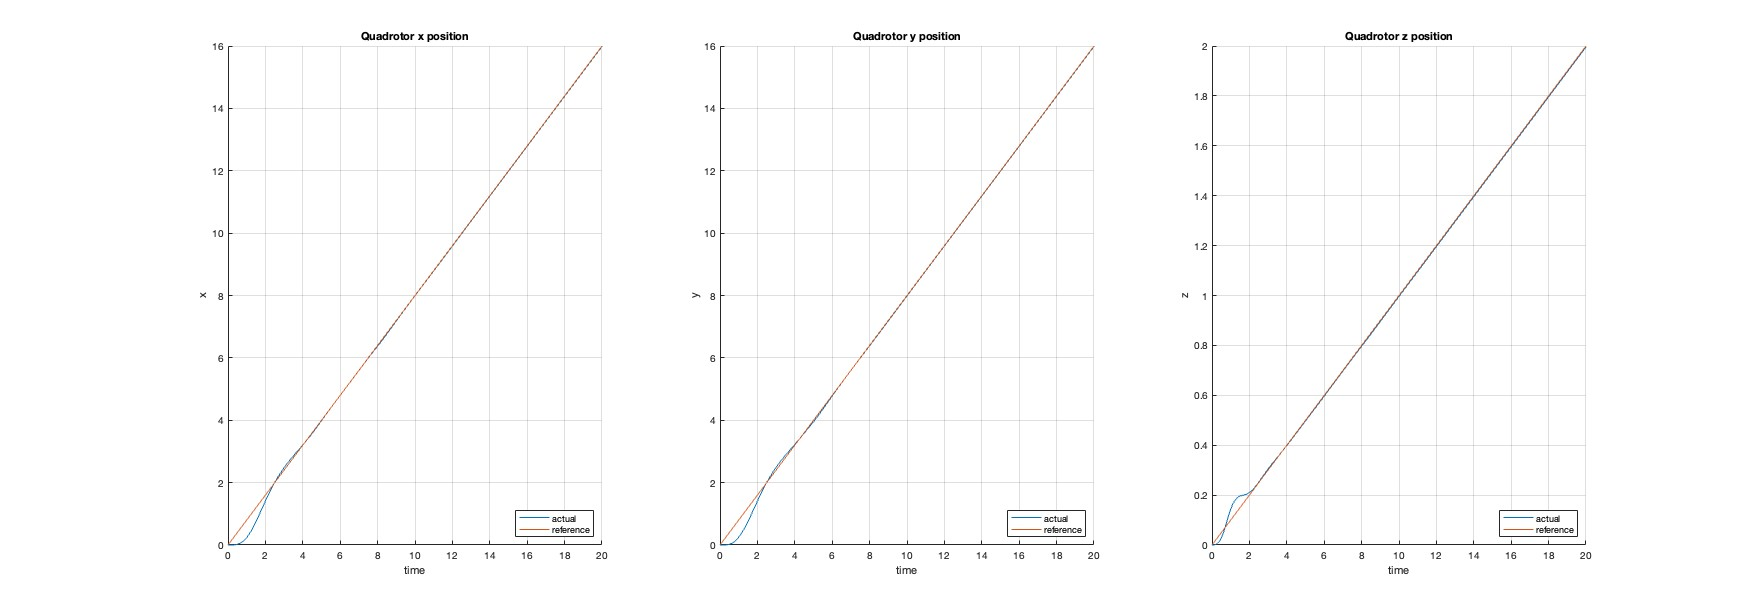
\includegraphics[width=.8\linewidth]{figures/mpc_evaluation_simple_path}
%     \caption{Drone position against simple reference path using MPC control }
%     \label{fig:mpc_evaluation_simple_path}
% \end{figure}

% \begin{figure}[H]
%     \centering
%     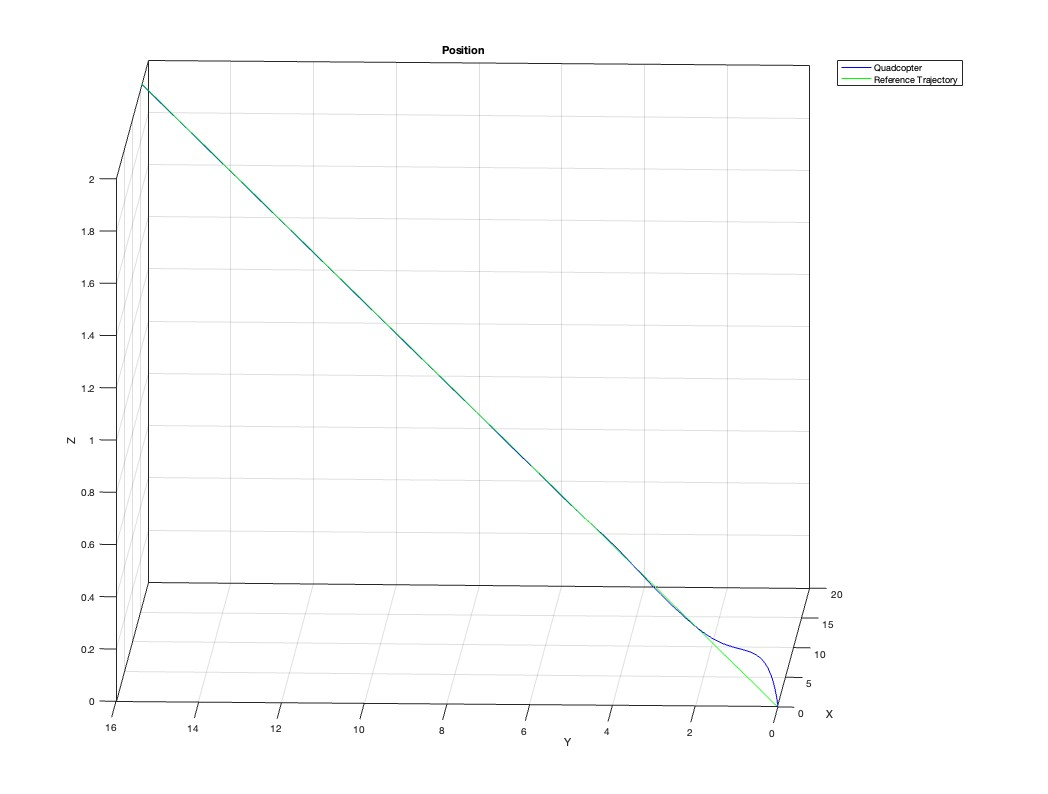
\includegraphics[width=.7\linewidth]{figures/mpc_simple_path}
%     \caption{Visualized drone flight path against simple reference path using MPC control }
%     \label{fig:mpc_simple_path}
% \end{figure}

We first evaluate out MPC control implementation using a complex spiral shaped path with no external wind. The result in Figure \ref{fig:mpc_evaluation_complex_path} and \ref{fig:mpc_complex_path}
shows that the quadcopter is able to track the reference path really well with close to zero overshooting

\begin{figure}[H]
    \centering
    \begin{subfigure}{.6\linewidth}
        \centering
        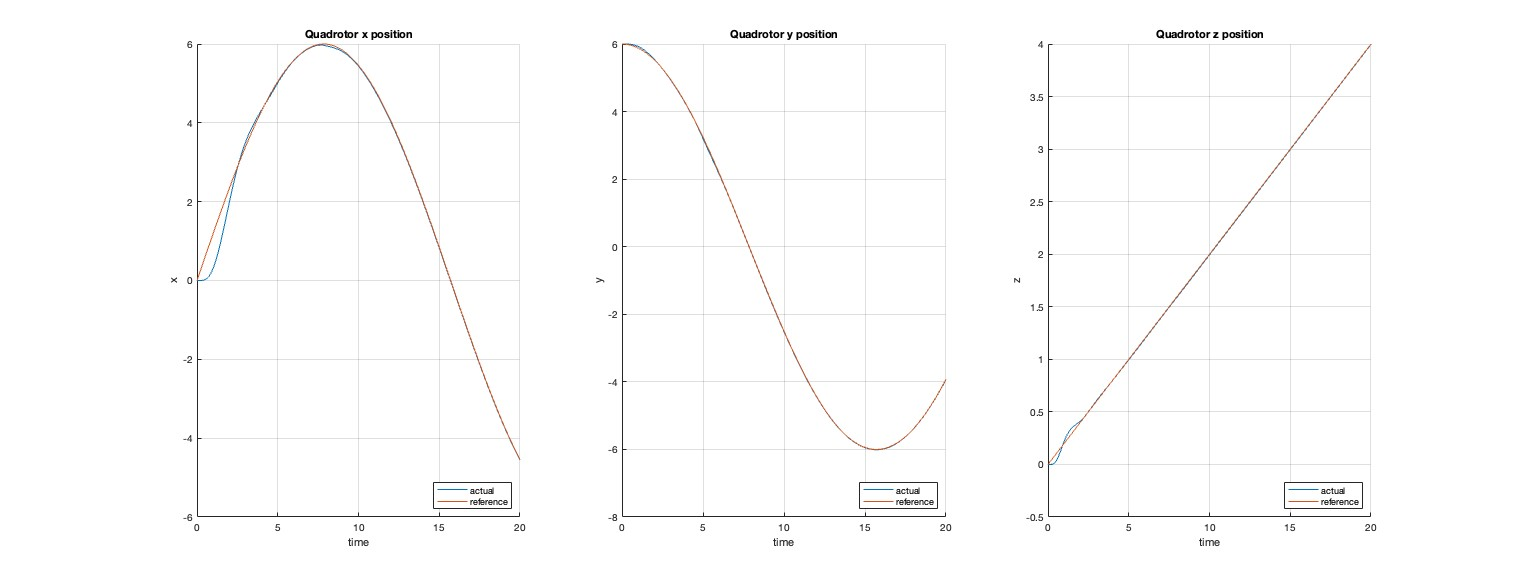
\includegraphics[width=\linewidth]{figures/mpc_evaluation_complex_path}
        \caption{Drone position against complex reference path }
        \label{fig:mpc_evaluation_complex_path}
    \end{subfigure}
    \begin{subfigure}{.35\linewidth}
        \centering
        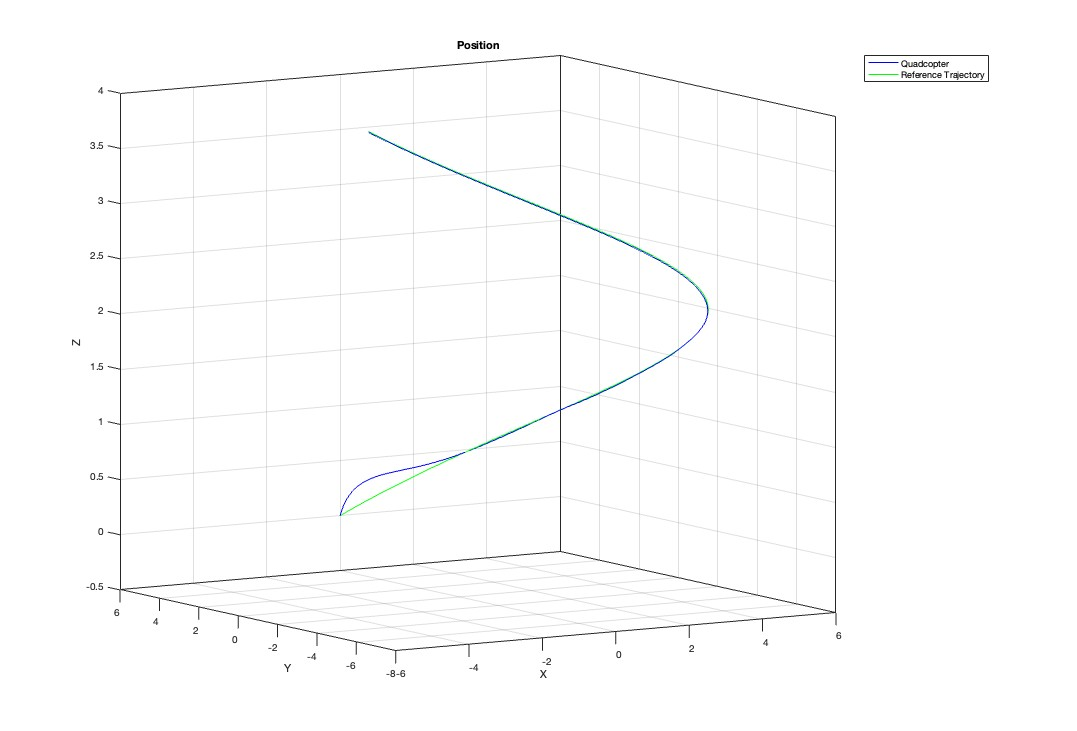
\includegraphics[width=\linewidth]{figures/mpc_complex_path}
        \caption{Visualized drone flight path}
        \label{fig:mpc_complex_path}
    \end{subfigure}
    \caption{MPC control evaluation against complex reference path}
\end{figure}

Finally we evaluate the MPC control with external wind disturbance.
The wind disturbance setup is as following:

\begin{itemize}
    \item horizonal wind present in $\hat{x}$ direction from 1-5s
    \item horizonal wind present in $\hat{y}$ direction from 5-8s
    \item horizonal wind with equal strength present in both $\hat{x}$ and $\hat{y}$ direction since 8s onwards
\end{itemize}

The simulation is done using the same  path shown in Figure \ref{fig:mpc_complex_path}.
We found that our MPC control can handle Strong Breeze condition well \cite{us_department_of_commerce_estimating_nodate}.
Its flight trajectory \ref{fig:mpc_evaluation_complex_path_strong_wind} is close to \ref{fig:mpc_complex_path} even under strong wind condition.
It is only under extreme wind condition like Near Gate (Inconvenience felt when walking against the wind) \cite{us_department_of_commerce_estimating_nodate},
MPC control will start to deviate from the reference path (Figure \ref{fig:mpc_complex_path_extreme_wind}). But this is more due to reaching the max thrust output limit of our model.

Overall, we think our MPC control method can control the quadcopter flight path quite satisfyingly under challenging wind conditions,

\begin{figure}[H]
    \centering
    \begin{subfigure}{.6\linewidth}
        \centering
        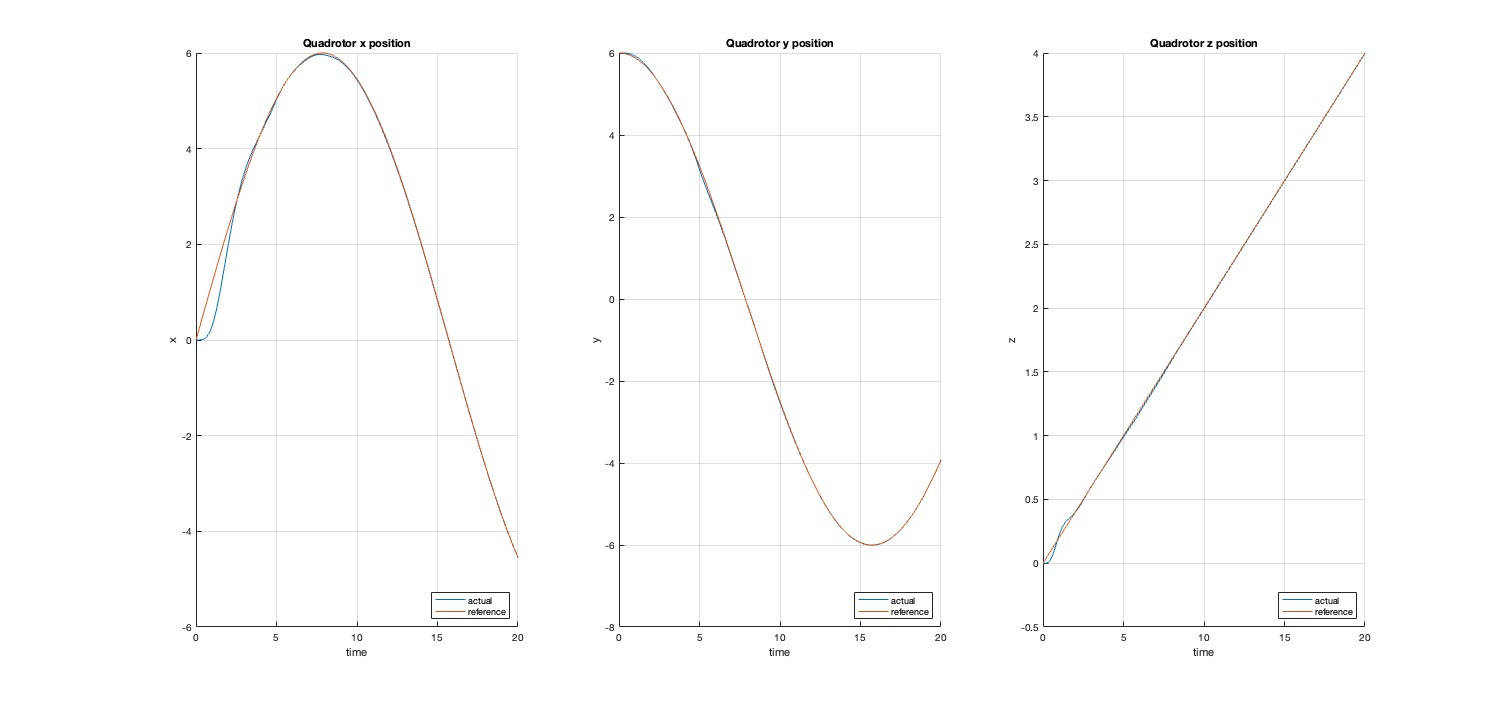
\includegraphics[width=\linewidth]{figures/mpc_evaluation_complex_path_strong_wind}
        \caption{Quadcopter position still tracks well under strong wind}
        \label{fig:mpc_evaluation_complex_path_strong_wind}
    \end{subfigure}
    \hspace{0.02\linewidth}
    \begin{subfigure}{.35\linewidth}
        \centering
        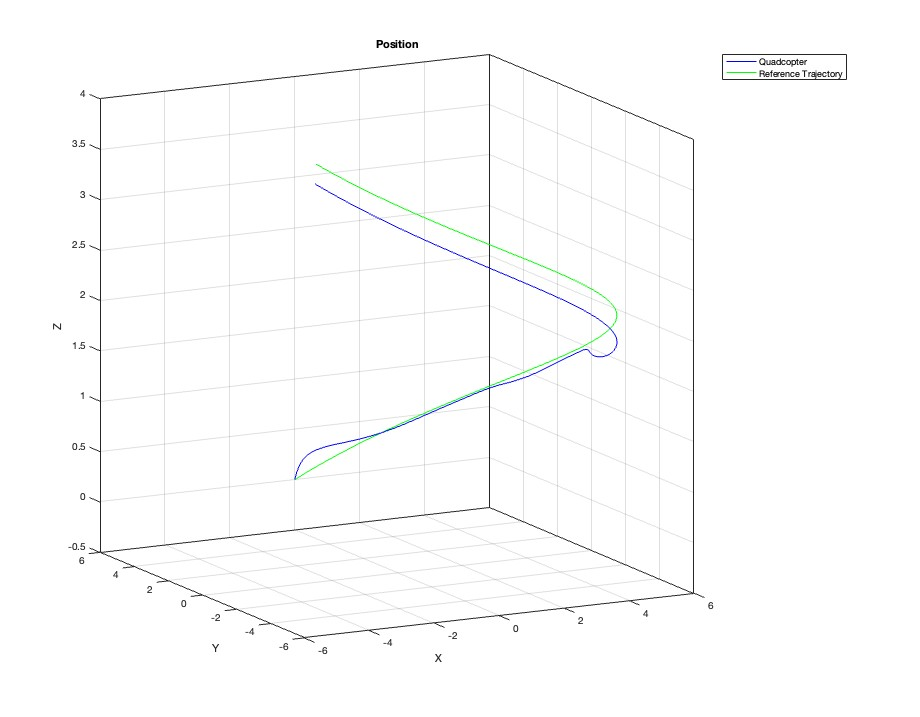
\includegraphics[width=\linewidth]{figures/mpc_complex_path_extreme_wind}
        \caption{Quadcopter fail to follow path under extreme windspeed}
        \label{fig:mpc_complex_path_extreme_wind}
    \end{subfigure}
    \caption{MPC control evaluation under different wind conditions}
\end{figure}

\section{[Sun Yijing]: Obstacle avoidance optimization algorithm}
\subsection{Improved Dijkstra's algorithm}

Inspired by Dijkstra's algorithm, I improved the Obstacle avoidance algorithm on its basis, which is similar to Dijkstra's algorithm, but uses heuristic functions to preferentially search points that are expected to be closer to the target point, usually Euclidean distance, thus reducing the calculation time. This algorithm can be basically divided into the following steps:
\begin{itemize}
    \item Initialize a fscore matrix that represents the estimated total cost from the starting point to the target point.
    \item Create an open collection, openset, that initially contains the starting point and sets its fscore.
    \item Iterate over and update the dist, prev, and fscore values of the neighbor nodes.
    \item Stop searching if the target point is reached.
\end{itemize}

\subsection{Minimum snap polynomial trajectory optimization}

At the same time, by minimizing the fourth derivative of acceleration (snap), we can optimize the polynomial trajectory given the starting point and end point, velocity, acceleration and acceleration conditions.
By constructing such an optimization problem, we can use the quadratic programming algorithm to find the optimal coefficient p, making the trajectory as smooth as possible, that is, minimizing the integral of the acceleration over the entire path.
Consider a polynomial $P$ of degree 9 such that:

\begin{equation}
    P(t) = p_9t^9 + p_8t^8 + \ldots + p_1t + p_0
\end{equation}

Since input $u_2$ and $u_3$ have up to 4th derivative (snap) of the positions, we are interested in optimizing $P$ by minimizing snap. Cost function $J$ can be written as:

\begin{equation}
    J = \int_0^T p^{(4)}(t)^2 dt = p^TQp
\end{equation}

Where $p$ is a column vector of the coefficients of the polynomial and $Q$ is a cost matrix. Now we present equality constraints in a form of:

\begin{equation}
    Ap = b, \quad b = \begin{bmatrix}
        x_0 & \dot{x}_0 & \ddot{x}_0 & \dddot{x}_0 & \ddddot{x}_0 \\
        x_T & \dot{x}_T & \ddot{x}_T & \dddot{x}_T & \ddddot{x}_T
    \end{bmatrix}
\end{equation}

Now we have a standard quadratic programming (QP) problem.

\subsection{The result after optimizing the path}
In this part, I will show three resulting graphs from three maps. The blue dot is the starting point, the red dot is the end point, and the squares of different sizes are obstacles.
Take the first fig map1 for example: You need to find a path that is efficient and doesn't collide with green obstacles.
There are two different tracks between the starting point and the ending point, among which the track composed of discrete points is obtained by the optimized Dijkstra algorithm, and the track composed of continuous line segments is obtained by further optimization method, like minimum snap polynomial trajectory optimization. Finally, there is a cost function to estimate the cost of the planned trajectory.
\begin{figure}[H]
    \centering
    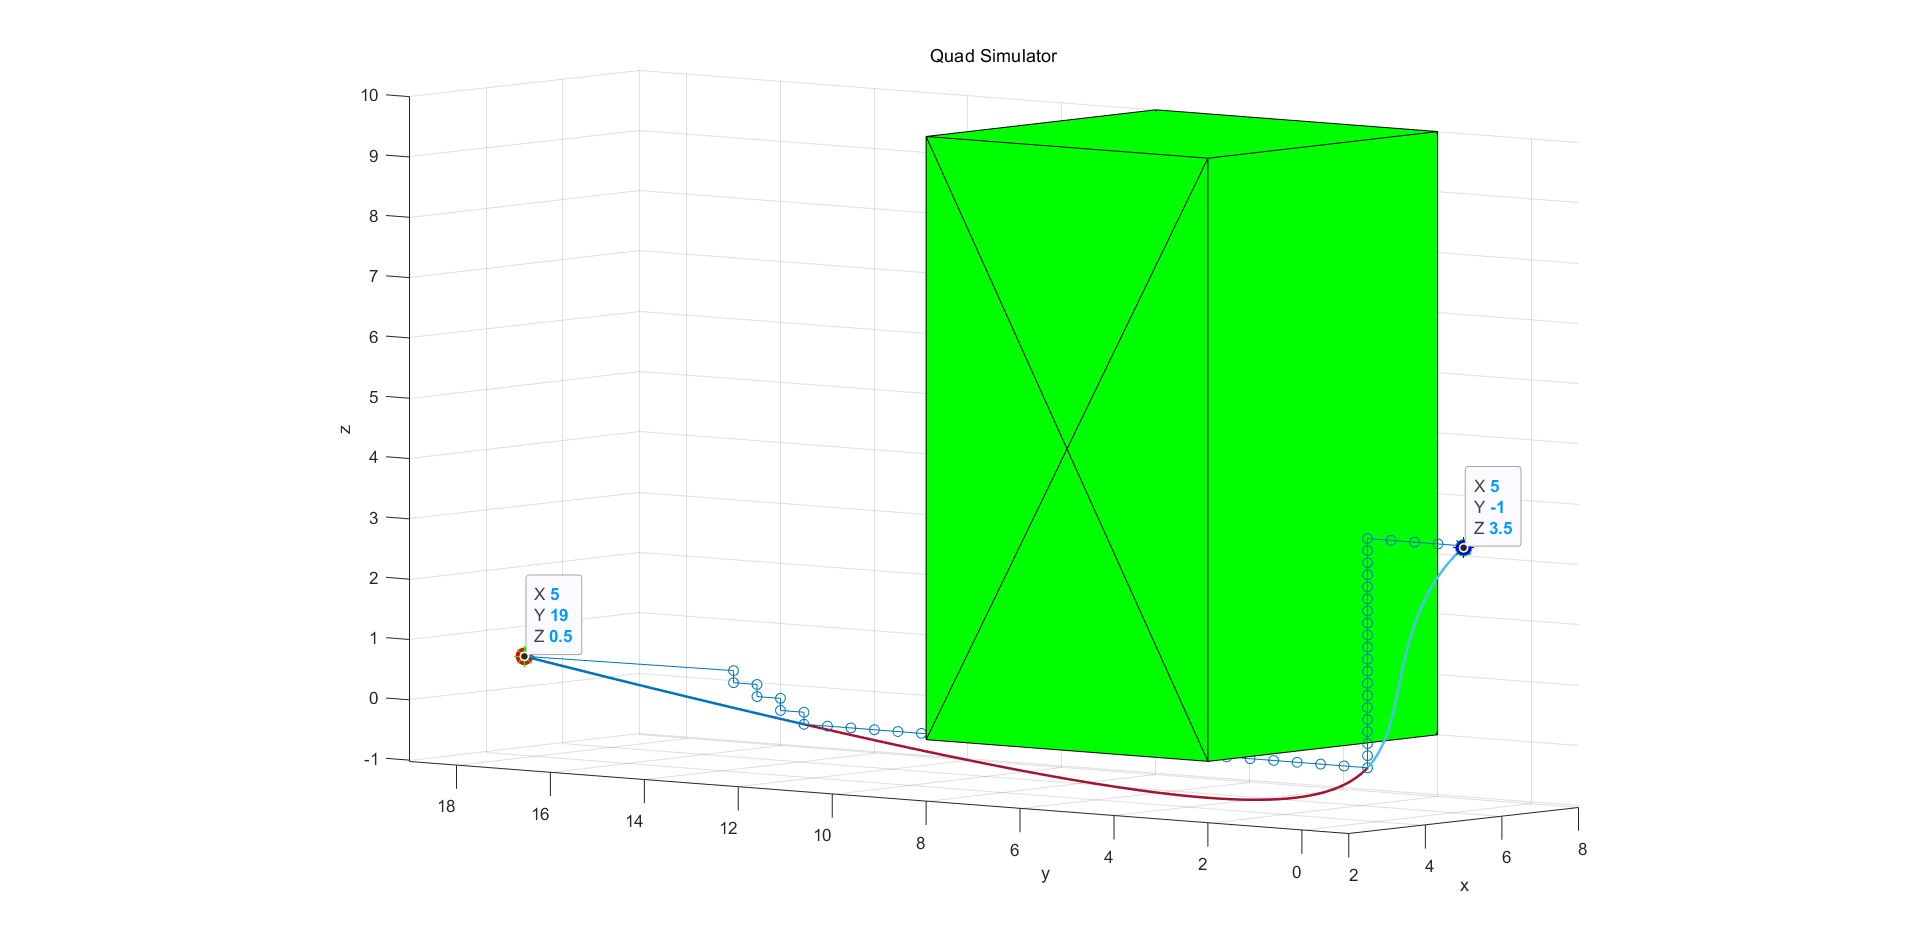
\includegraphics[width=.8\linewidth]{figures/map1}
    \caption{The result after optimizing the path in map1}
\end{figure}
The remaining two figures are shown below. They are similar to the results in the first image. The optimized trajectory successfully bypasses all obstacles and reaches the end point.
The further optimized trajectories are smoother, safer and better able to avoid obstacles, because when calculating trajectories, I increase reliability by inflating the volume of obstacles to ensure that the trajectories do not collide with obstacles when detecting collisions. At the same time, a trajectory consisting of continuous line segments costs less and is more efficient. Even in the more complex environment as shown in Map 3, the algorithm can complete the trajectory planning properly.
However, this algorithm has not been combined with the UAV model, and the parameter design is too complicated. I will further study it in project1
\begin{figure}[H]
    \centering
    \begin{subfigure}{.45\textwidth}
        \centering
        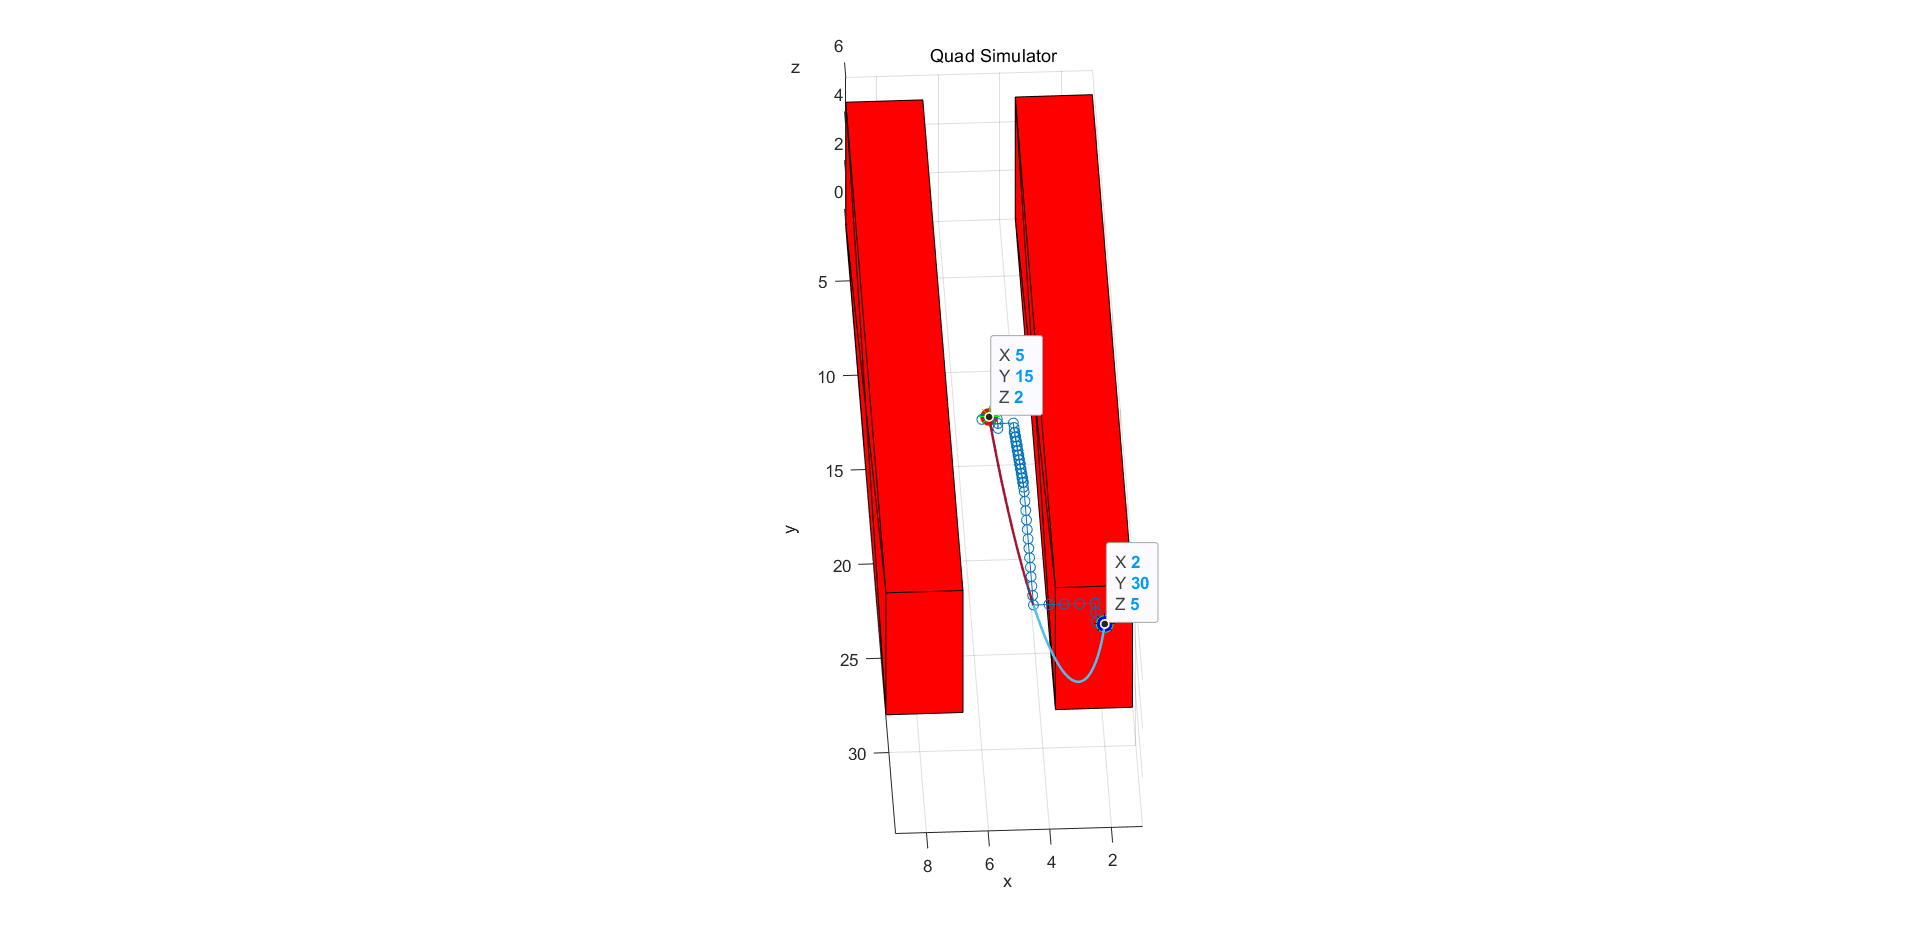
\includegraphics[width=\linewidth]{figures/map2}
        \caption{result in map2}
        \label{fig:optimized_path_map2}
    \end{subfigure}
    \hspace{.05\textwidth}  % This will ensure that the subfigures are spaced out to the full text width
    \begin{subfigure}{.45\textwidth}
        \centering
        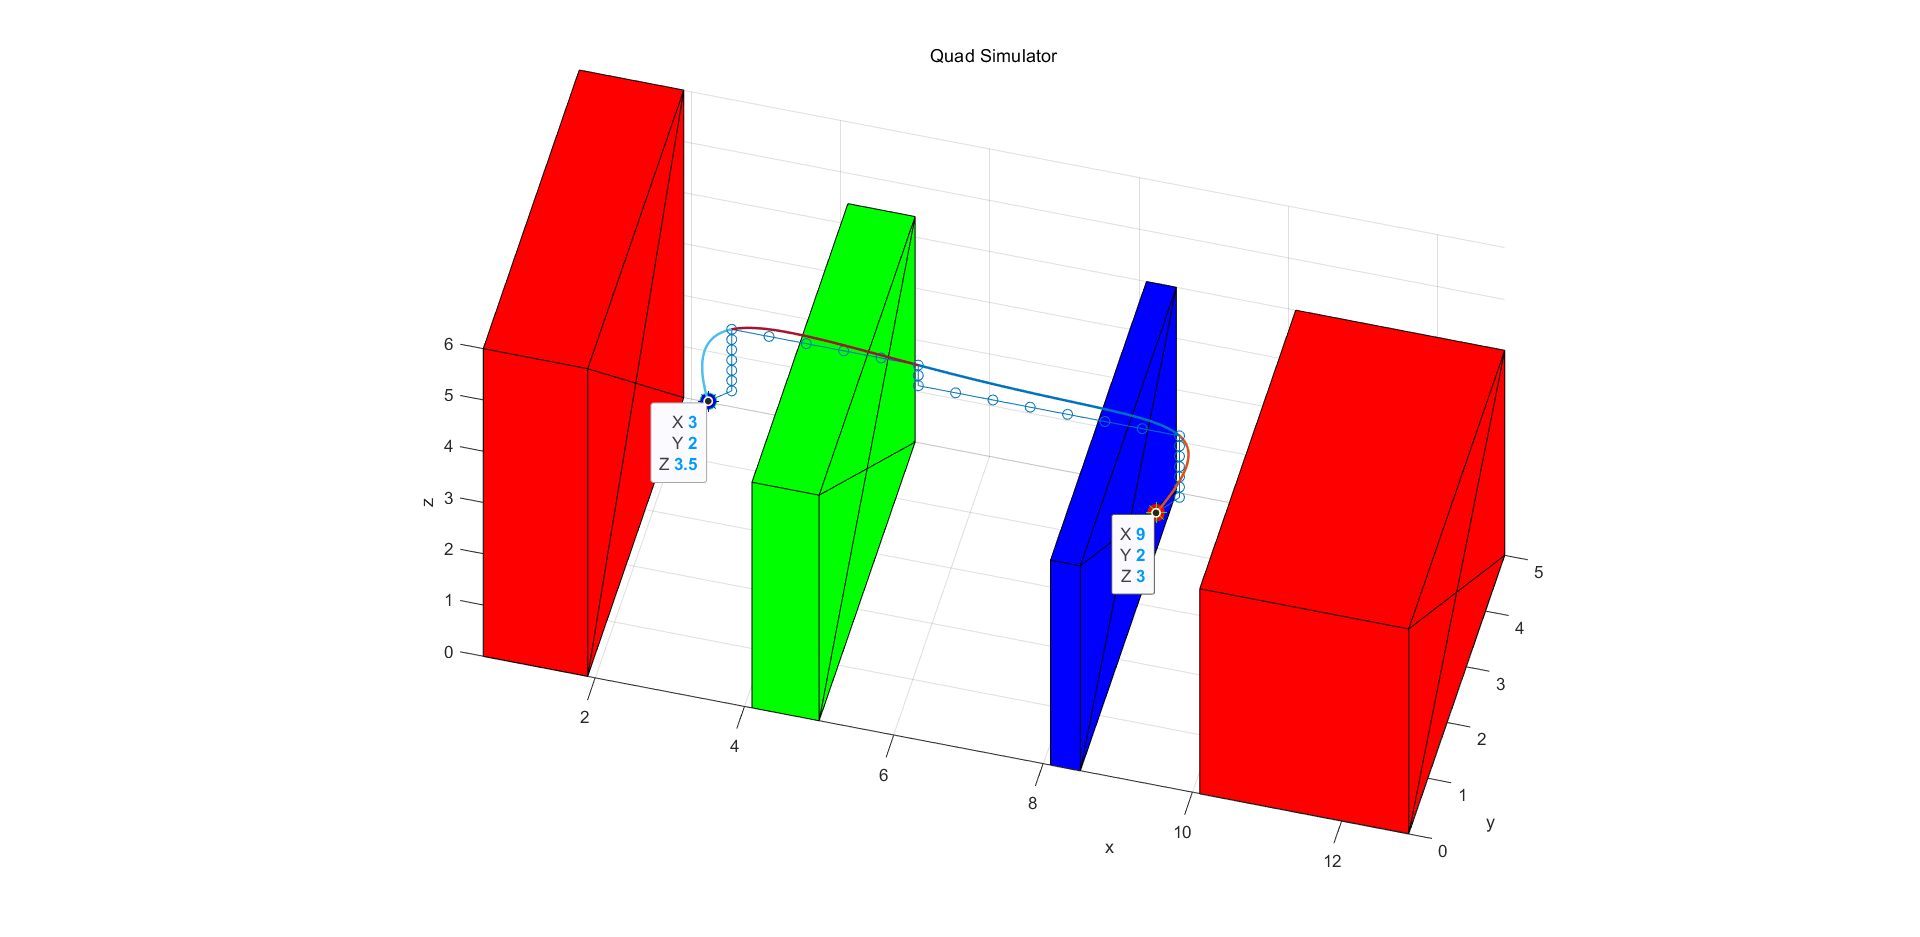
\includegraphics[width=\linewidth]{figures/map3}
        \caption{result in map3}
        \label{fig:optimized_path_map3}
    \end{subfigure}
    \caption{Results after optimizing the path in different maps}
    \label{fig:optimized_path_maps}
\end{figure}

\section{[Ma Haoyuan]: Plot Words with Trajectories}


Similar to how drones are used in light shows, plotting words or symbols could be used for advertising, entertainment, artistic displays, or various celebrations.
Besides, it can also be used to demonstrate drone control and programming in a visually engaging way.
In my work, a simplified flight path that spells out the word "NUS" is designed and simulated.

\subsection{Generation of Quadcoper's Target Reference Points}
In order to plot the word "NUS", or any other words in the future, we need to design and specify the target trace points for each character firstly, which can be used subsequently to direct the drone.

To achieve the goal, I designed the character pattern in a top-down 2D view for simplicity as the first step, as shown in the following figure:
\begin{figure}[H]
    \centering
    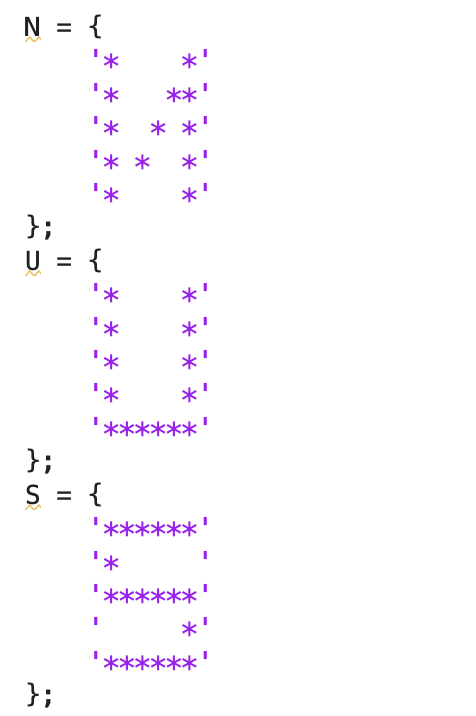
\includegraphics[width=.2\linewidth]{figures/nus_word_pattern}
    \caption{Visualized 2D view pattern for word "NUS" }
    \label{fig:nus_word_pattern}
\end{figure}

Then, we derive the trace points manually for each character. During this procedure, we only care about the relative coordination value(since it can be later scaled up or down simply) and assume that their z-axis coordination values equal to 0(can be later changed using bias):
\begin{lstlisting}[language=Matlab, basicstyle=\tiny]
    charPositionMap('N') = [0, 1, 0; 0, 0, 0; 1, 1, 0; 1, 0, 0] + positionBias;
    charPositionMap('U') = [0, 1, 0; 0, 0, 0; 1, 0, 0; 1, 1, 0] + positionBias;
    charPositionMap('S') = [1, 1, 0; 0, 1, 0; 0, 0.5, 0; 1, 0.5, 0; 1, 0, 0; 0, 0, 0] + positionBias;
\end{lstlisting}

Next step is the construction of global trace points, during which their values are scaled with given factor.


\subsection{Directing Quadcoper to Plot Words in 3D-Space}
In this part, I will show you the simulation results which aims to direct the quadcoper to plot the word "NUS" through its trajectories with different views:

\begin{figure}[H]
    \centering
    \begin{subfigure}{.45\textwidth}
        \centering
        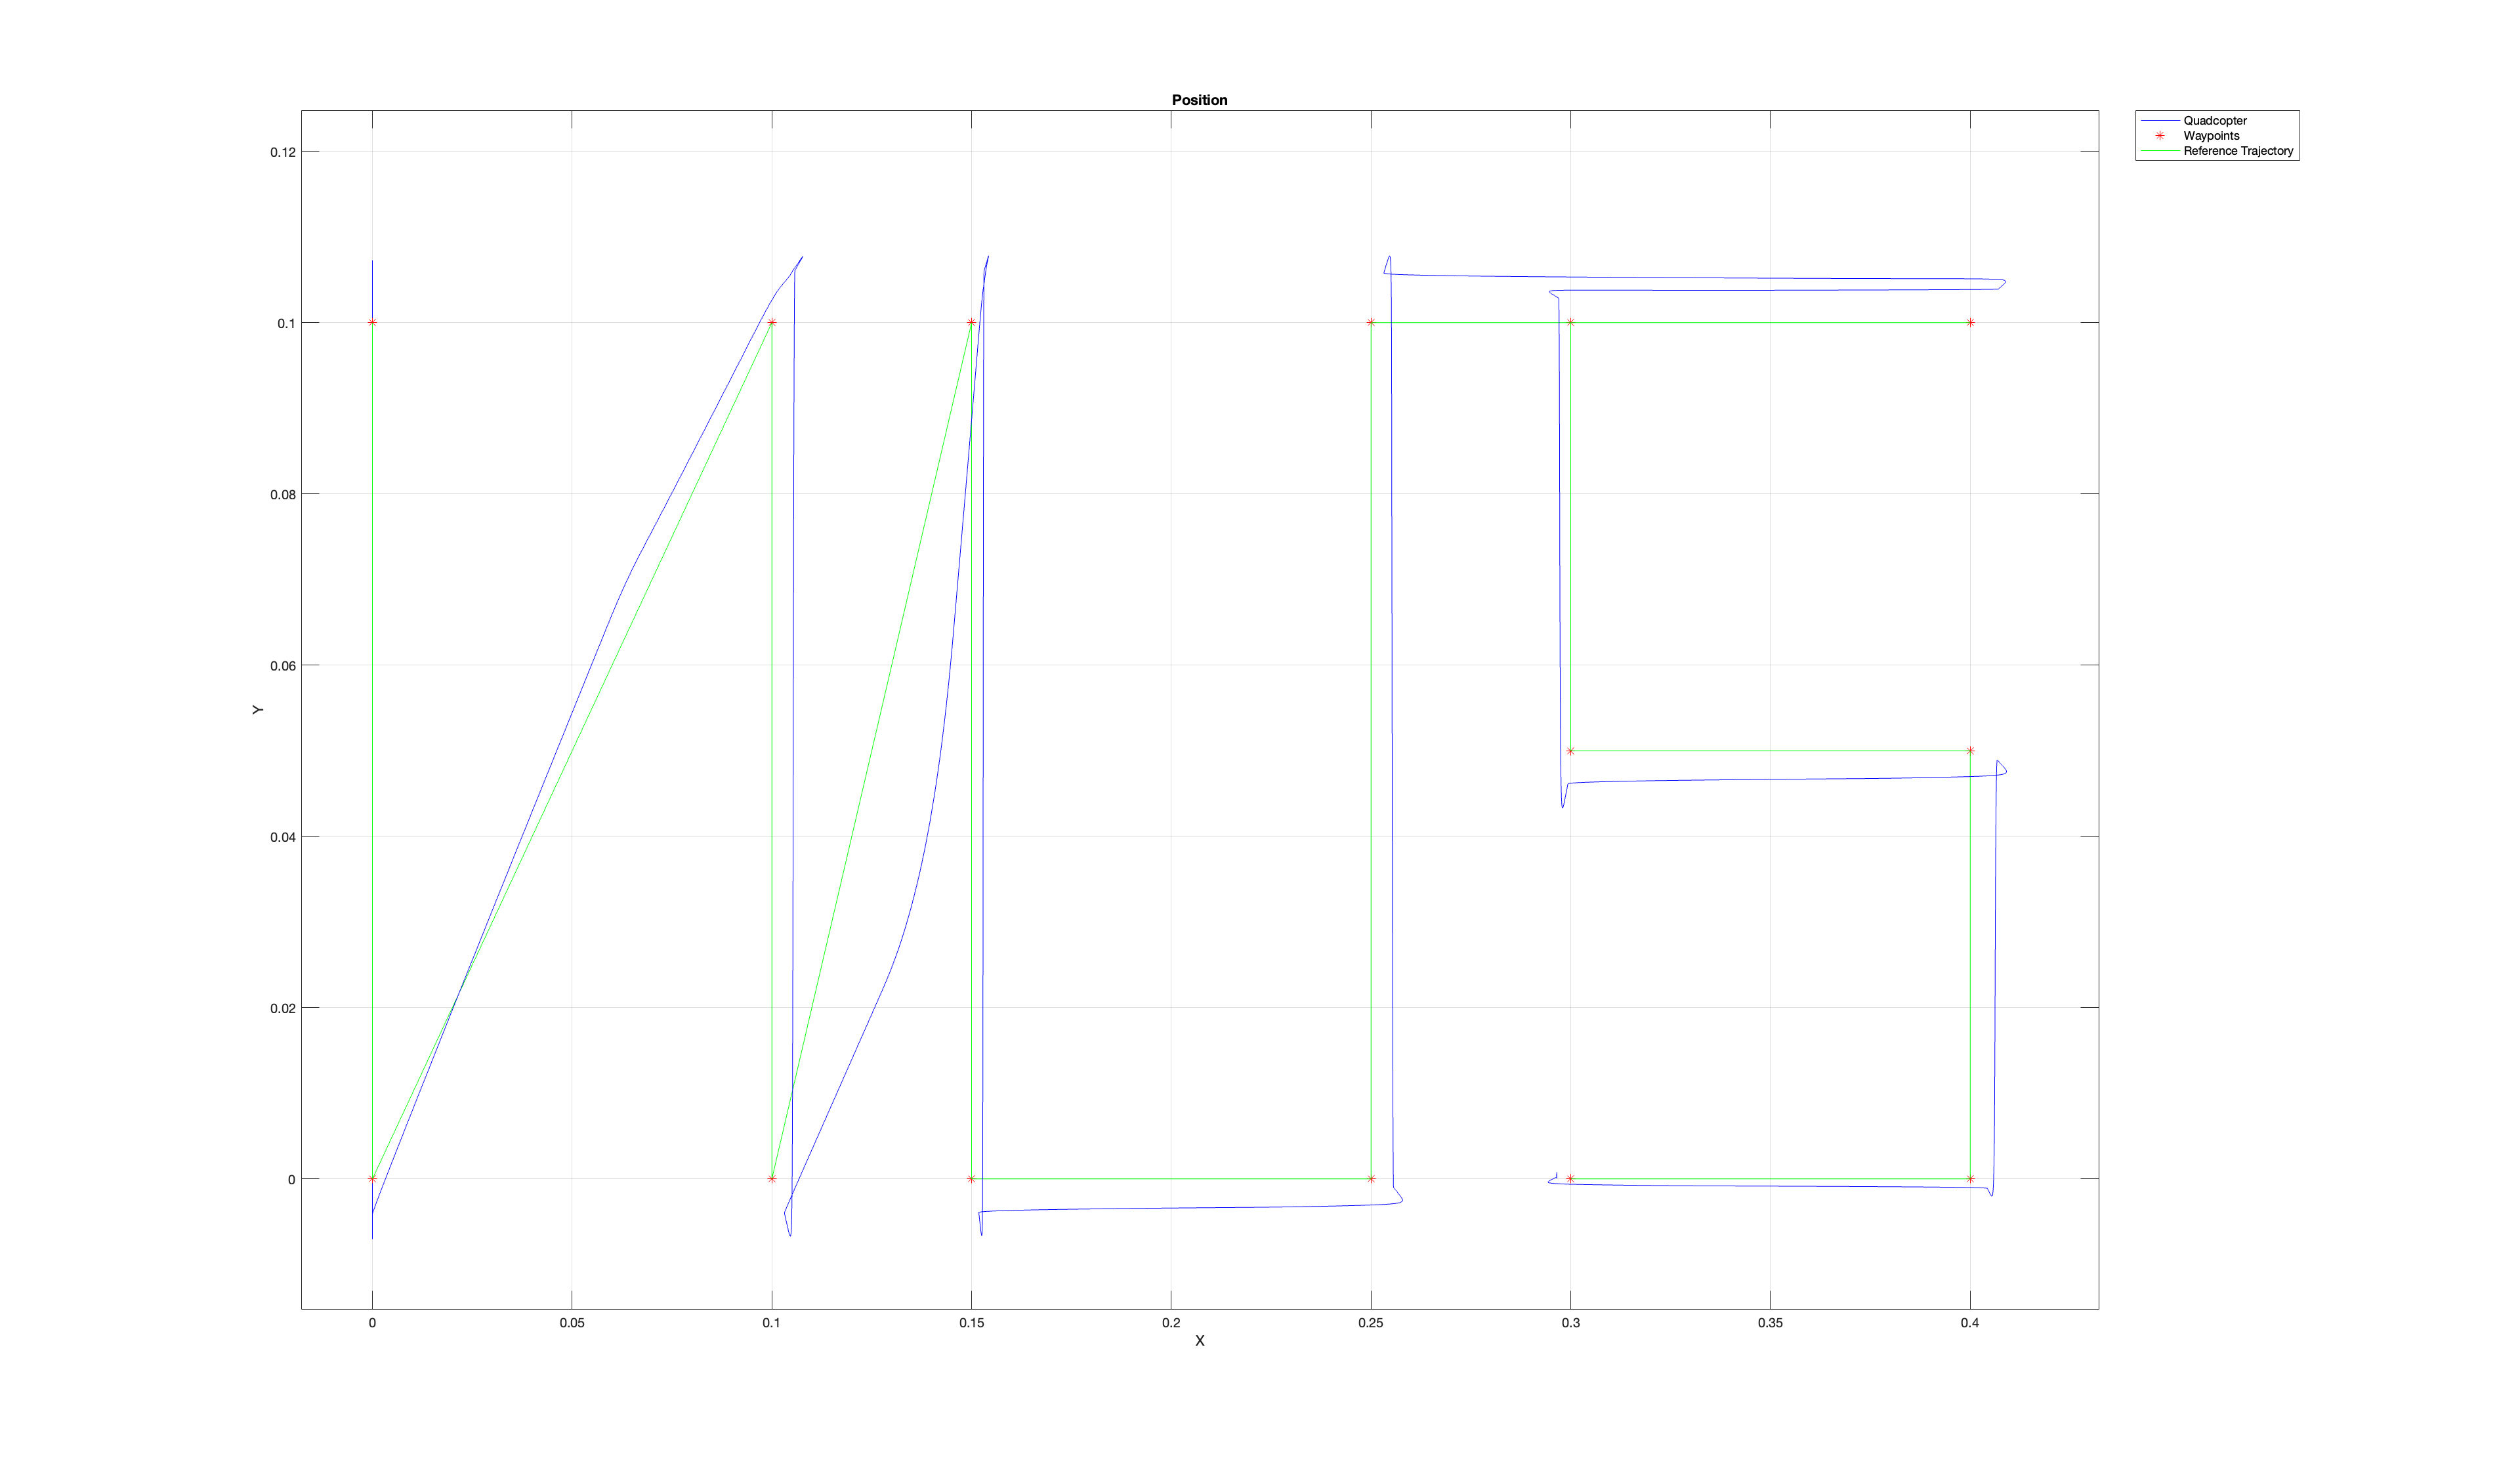
\includegraphics[width=\linewidth]{figures/nus_word_top_down_view}
        \caption{Top-Down view}
        \label{fig:nus_word_top_down_view}
    \end{subfigure}
    \hspace{.05\textwidth}  % This will ensure that the subfigures are spaced out to the full text width
    \begin{subfigure}{.45\textwidth}
        \centering
        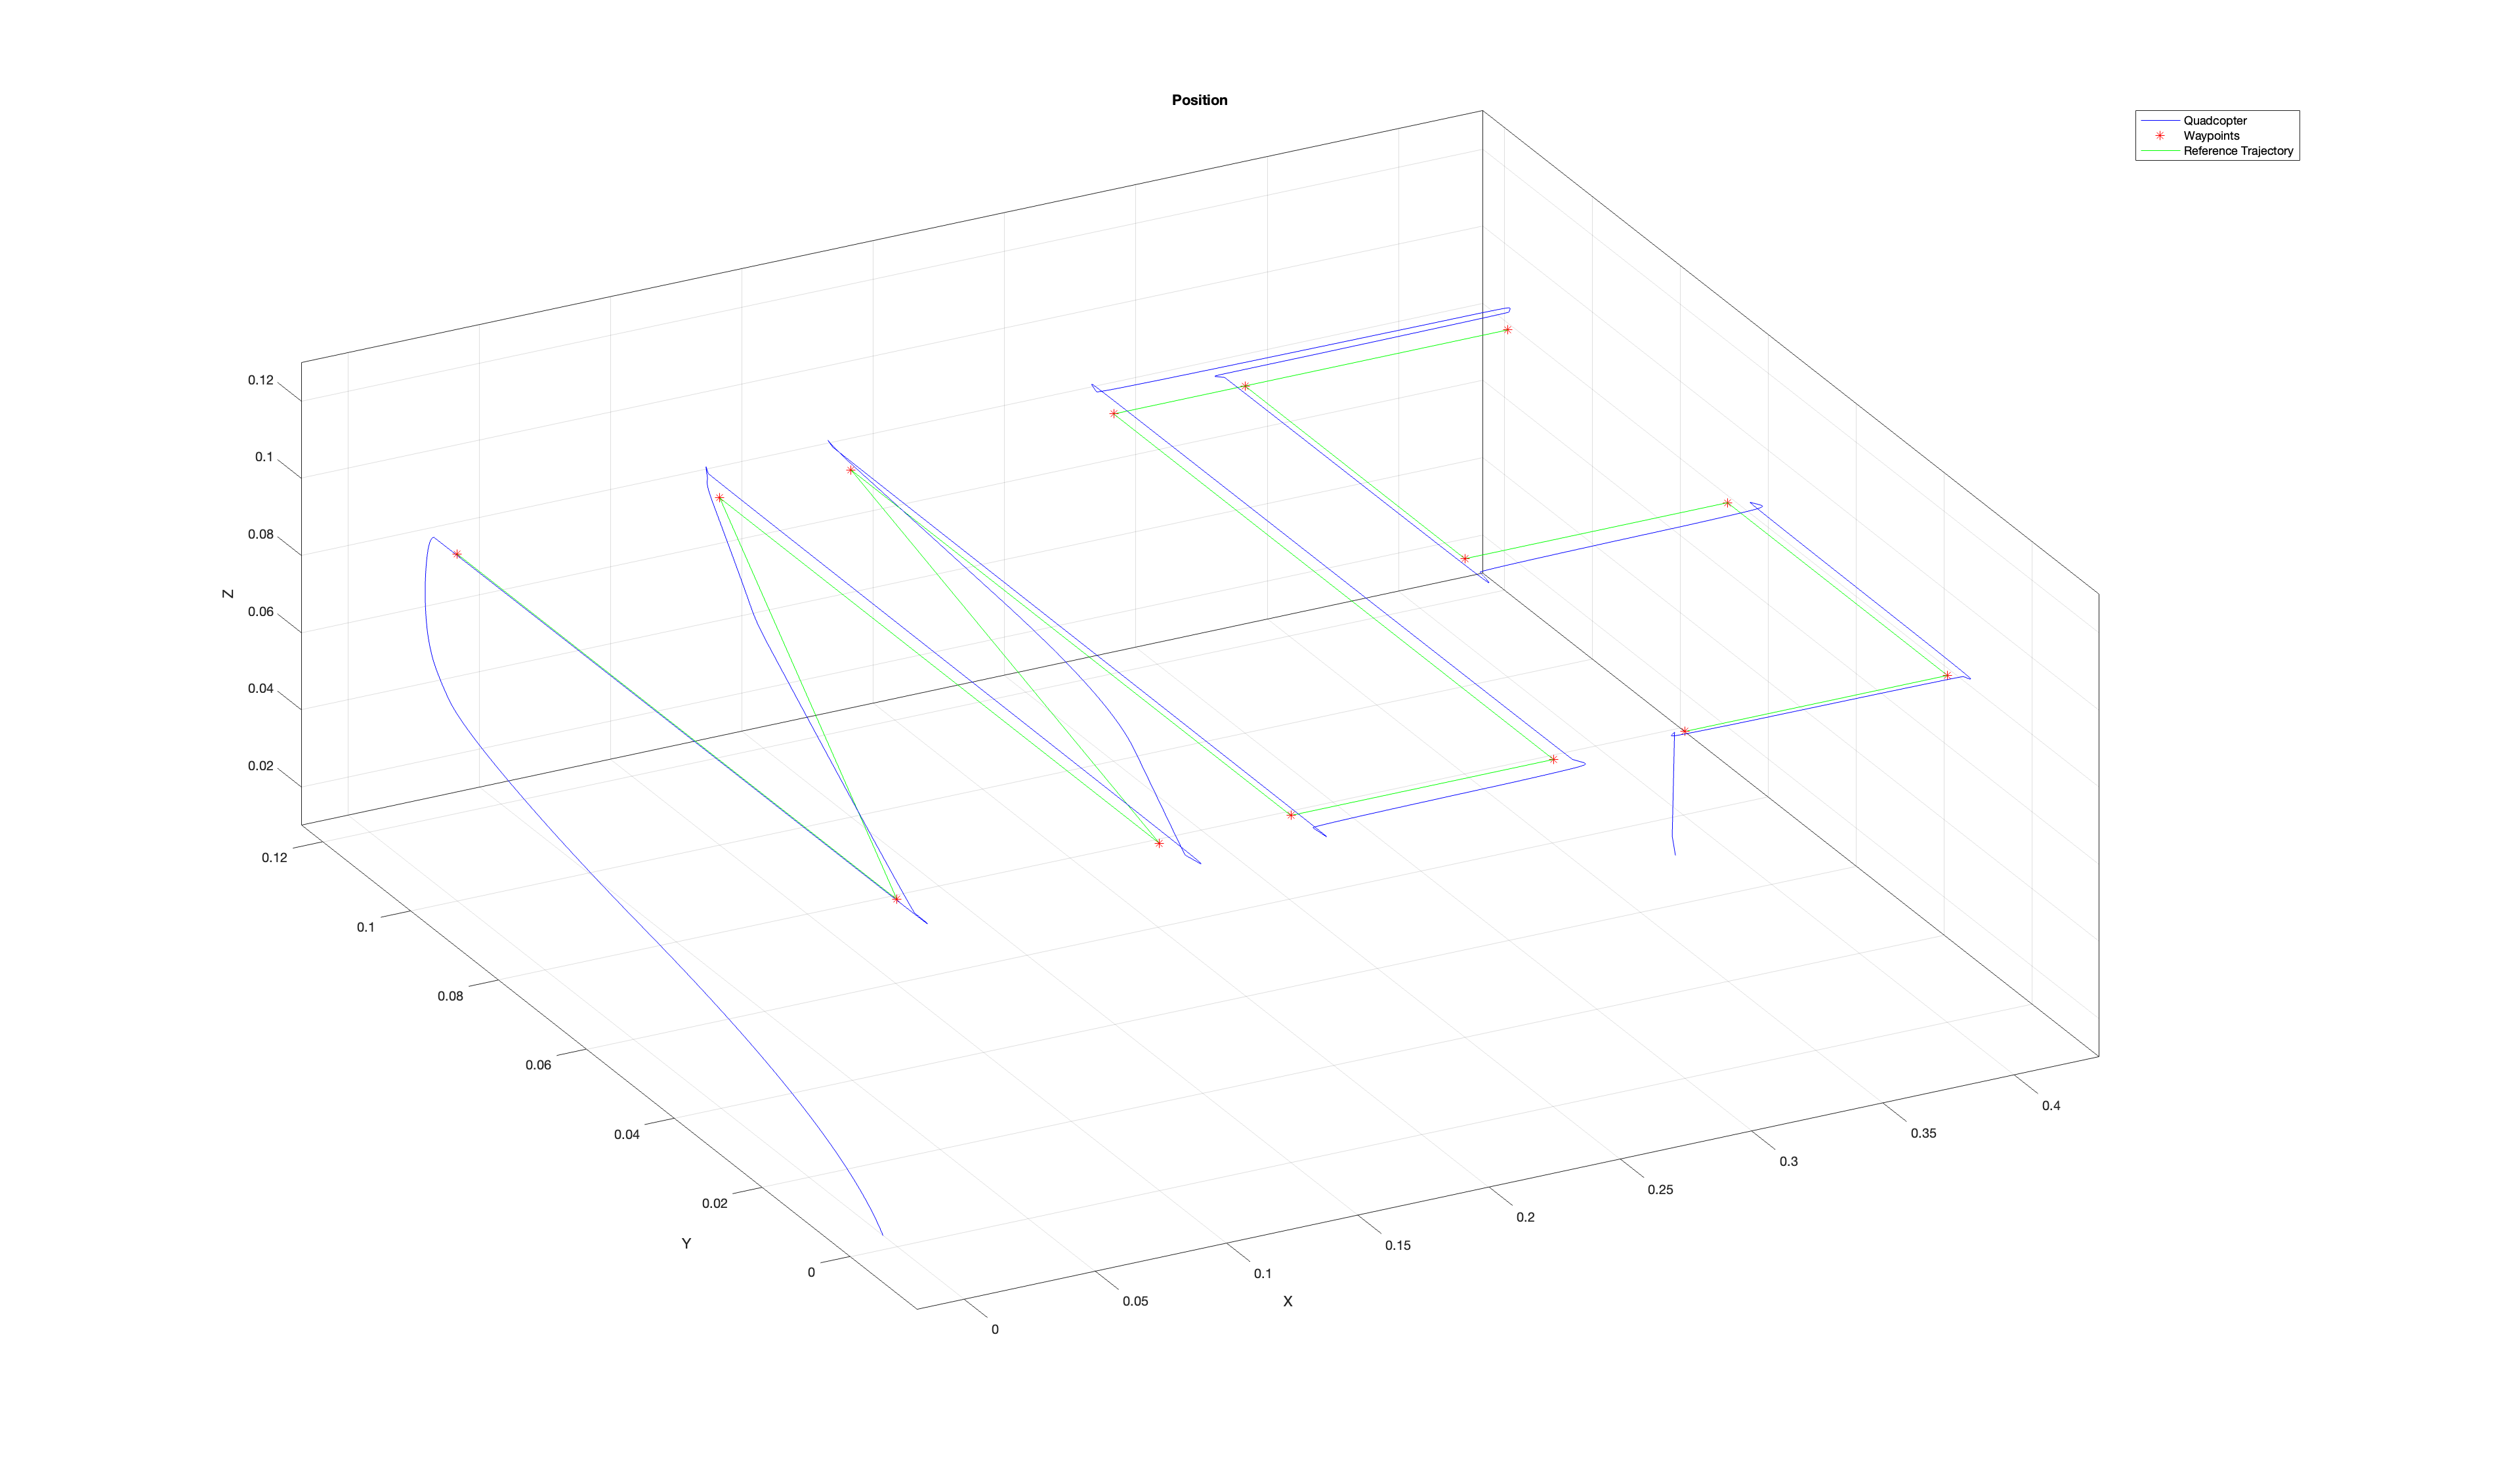
\includegraphics[width=\linewidth]{figures/nus_word_3d_space_view}
        \caption{3D-space view}
        \label{fig:nus_word_3d_space_view}
    \end{subfigure}
    \caption{Visualized views of word "NUS" plotting by the quadcoper}
    \label{fig:nus_word_views}
\end{figure}


As figures shown above, when using PID controller without wind model, results are quite acceptable though it's just a simplified simulation case. To further evaluate the performance of PID controller, the drone's position against reference trace points for 3 axis is also shown below:
\begin{figure}[H]
    \centering
    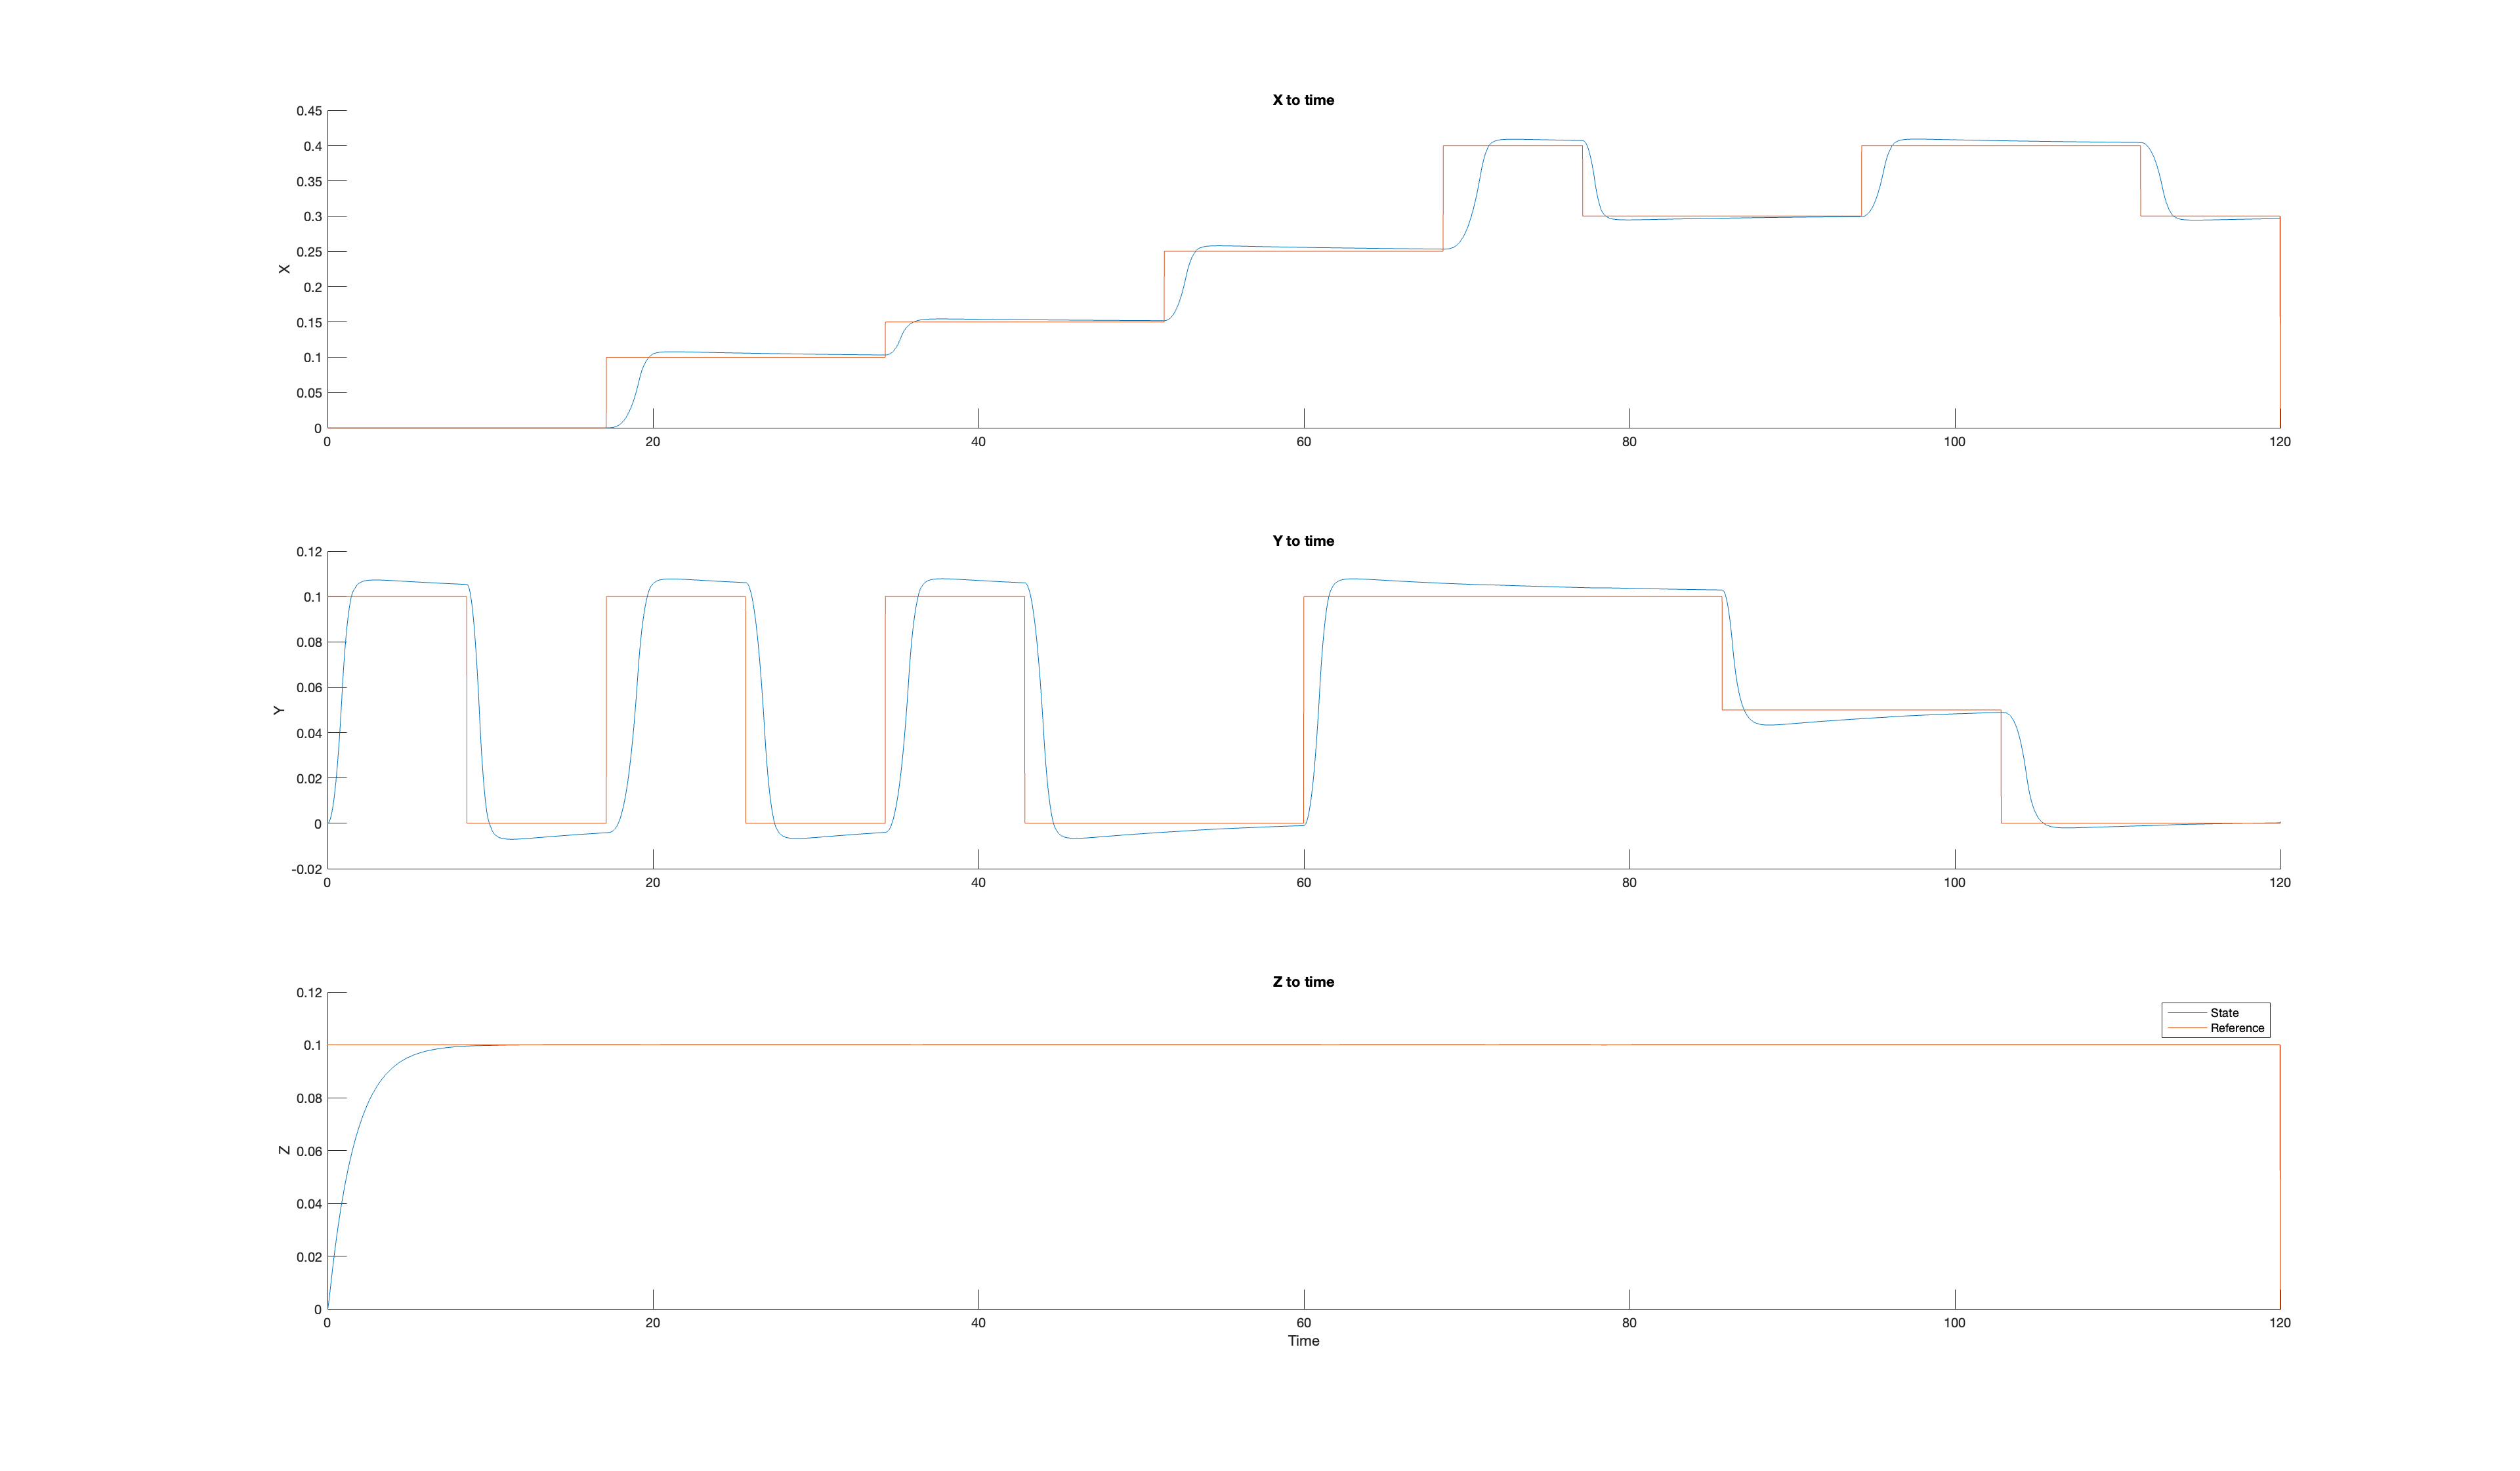
\includegraphics[width=.5\linewidth]{figures/nus_word_xyz}
    \caption{Quadcoper's 3-Axis position against reference trace points}
    \label{fig:nus_word_xyz}
\end{figure}

As we can see, though with some limitations and inaccuracy, the PID controller can indeed provide the acceptable control performance under this scenario, which again proves the effect, correctness, and value of our group's previous work.

\newpage
\pagenumbering{roman}
\bibliography{references}

\end{document}
